% SVN Info:
% $Date: 2021-01-29 22:28:41 +0100 (Fr, 29 Jan 2021) $
% $Rev: 1039 $
% $Author: kolja $
\lstset{
	language=[Visual]C++,
	keywordstyle=\bfseries\sffamily\color[rgb]{0,0,1},
	identifierstyle=\sffamily,
	commentstyle=\color[rgb]{0.133,0.545,0.133},
	stringstyle=\sffamily\color[rgb]{0.627,0.126,0.941},
	showstringspaces=false,
	basicstyle=\small,
	numberstyle=\footnotesize,
	numbers=left,
	stepnumber=1,
	numbersep=10pt,
	tabsize=2,
	breaklines=true,
	prebreak = \raisebox{0ex}[0ex][0ex]{\ensuremath{\hookleftarrow}},
	breakatwhitespace=false,
	aboveskip={1.5\baselineskip},
	columns=fixed,
	upquote=true,
	extendedchars=true,
}

\section{Installing the Board}
	%
	\balance
	%
The \deviceName\ board can be installed in any PCIe-CEM slot wiht x1 or more lanes. 
Make sure the PC is powered off and the main power connector is disconnected while installing the board.\par

%
\section{\deviceName\ Inputs and Connectors}
	\subsection{Connectors}
	%
	The inputs of the \deviceName\ are located on the slot bracket. Figure \ref{fig:schematics} on page \pageref{fig:schematics} shows the location of the start input S and the four stop inputs A to D.
%
	\begin{figure*}[hb]
		\begin{center}
			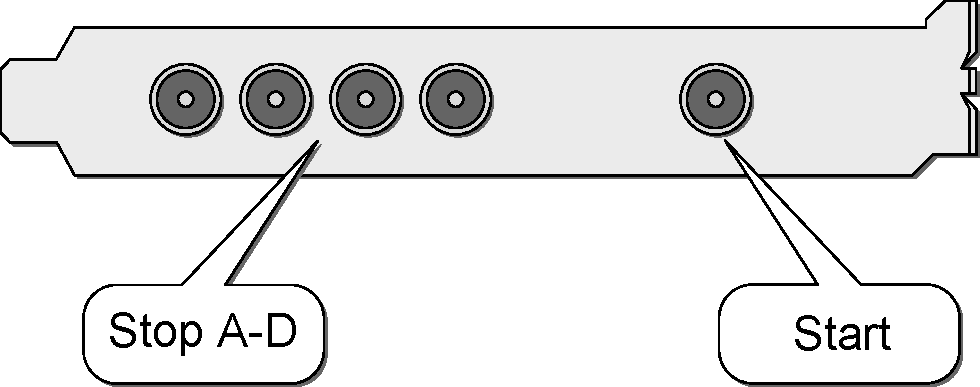
\includegraphics[width=0.6\textwidth]{figures/xTDC4_Slotblende.pdf}
			\caption{Input connectors of the \deviceName\ located on the PCIe bracket.}
		\end{center}
	\end{figure*}
	%
	%
		\begin{figure*}[hb]
			\begin{center}
				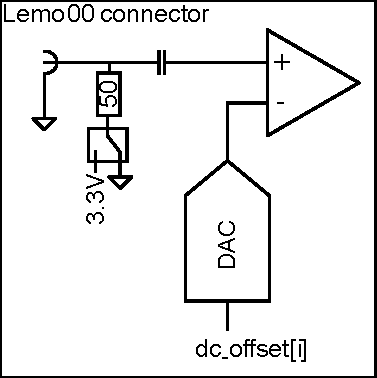
\includegraphics[width=0.3\textwidth]{figures/InputCircuit.pdf}
				\caption{Input circuit for each of the five input channels.\label{fig:inputcirc}}
			\end{center}
		\end{figure*}
		%
	Lemo-00 connectors are used for input connection. The inputs are AC-coupled and have an impedance of 50$\Omega$. 
	A schematic of the input circuit is shown in Figure \ref{fig:inputcirc} on page \pageref{fig:inputcirc}. 
	The digital threshold for any input can be adjusted in order to comply with a manifold of single ended signaling standards.
	The threshold can also be used to configure the input for either positive or negative pulses.
	
	The active termination can be used to generate DC-coupled output pulses for automatic internal triggering and control of external devices using the TiGer timing pattern generator.
	%
		\begin{figure*}[ht]
			\begin{center}
				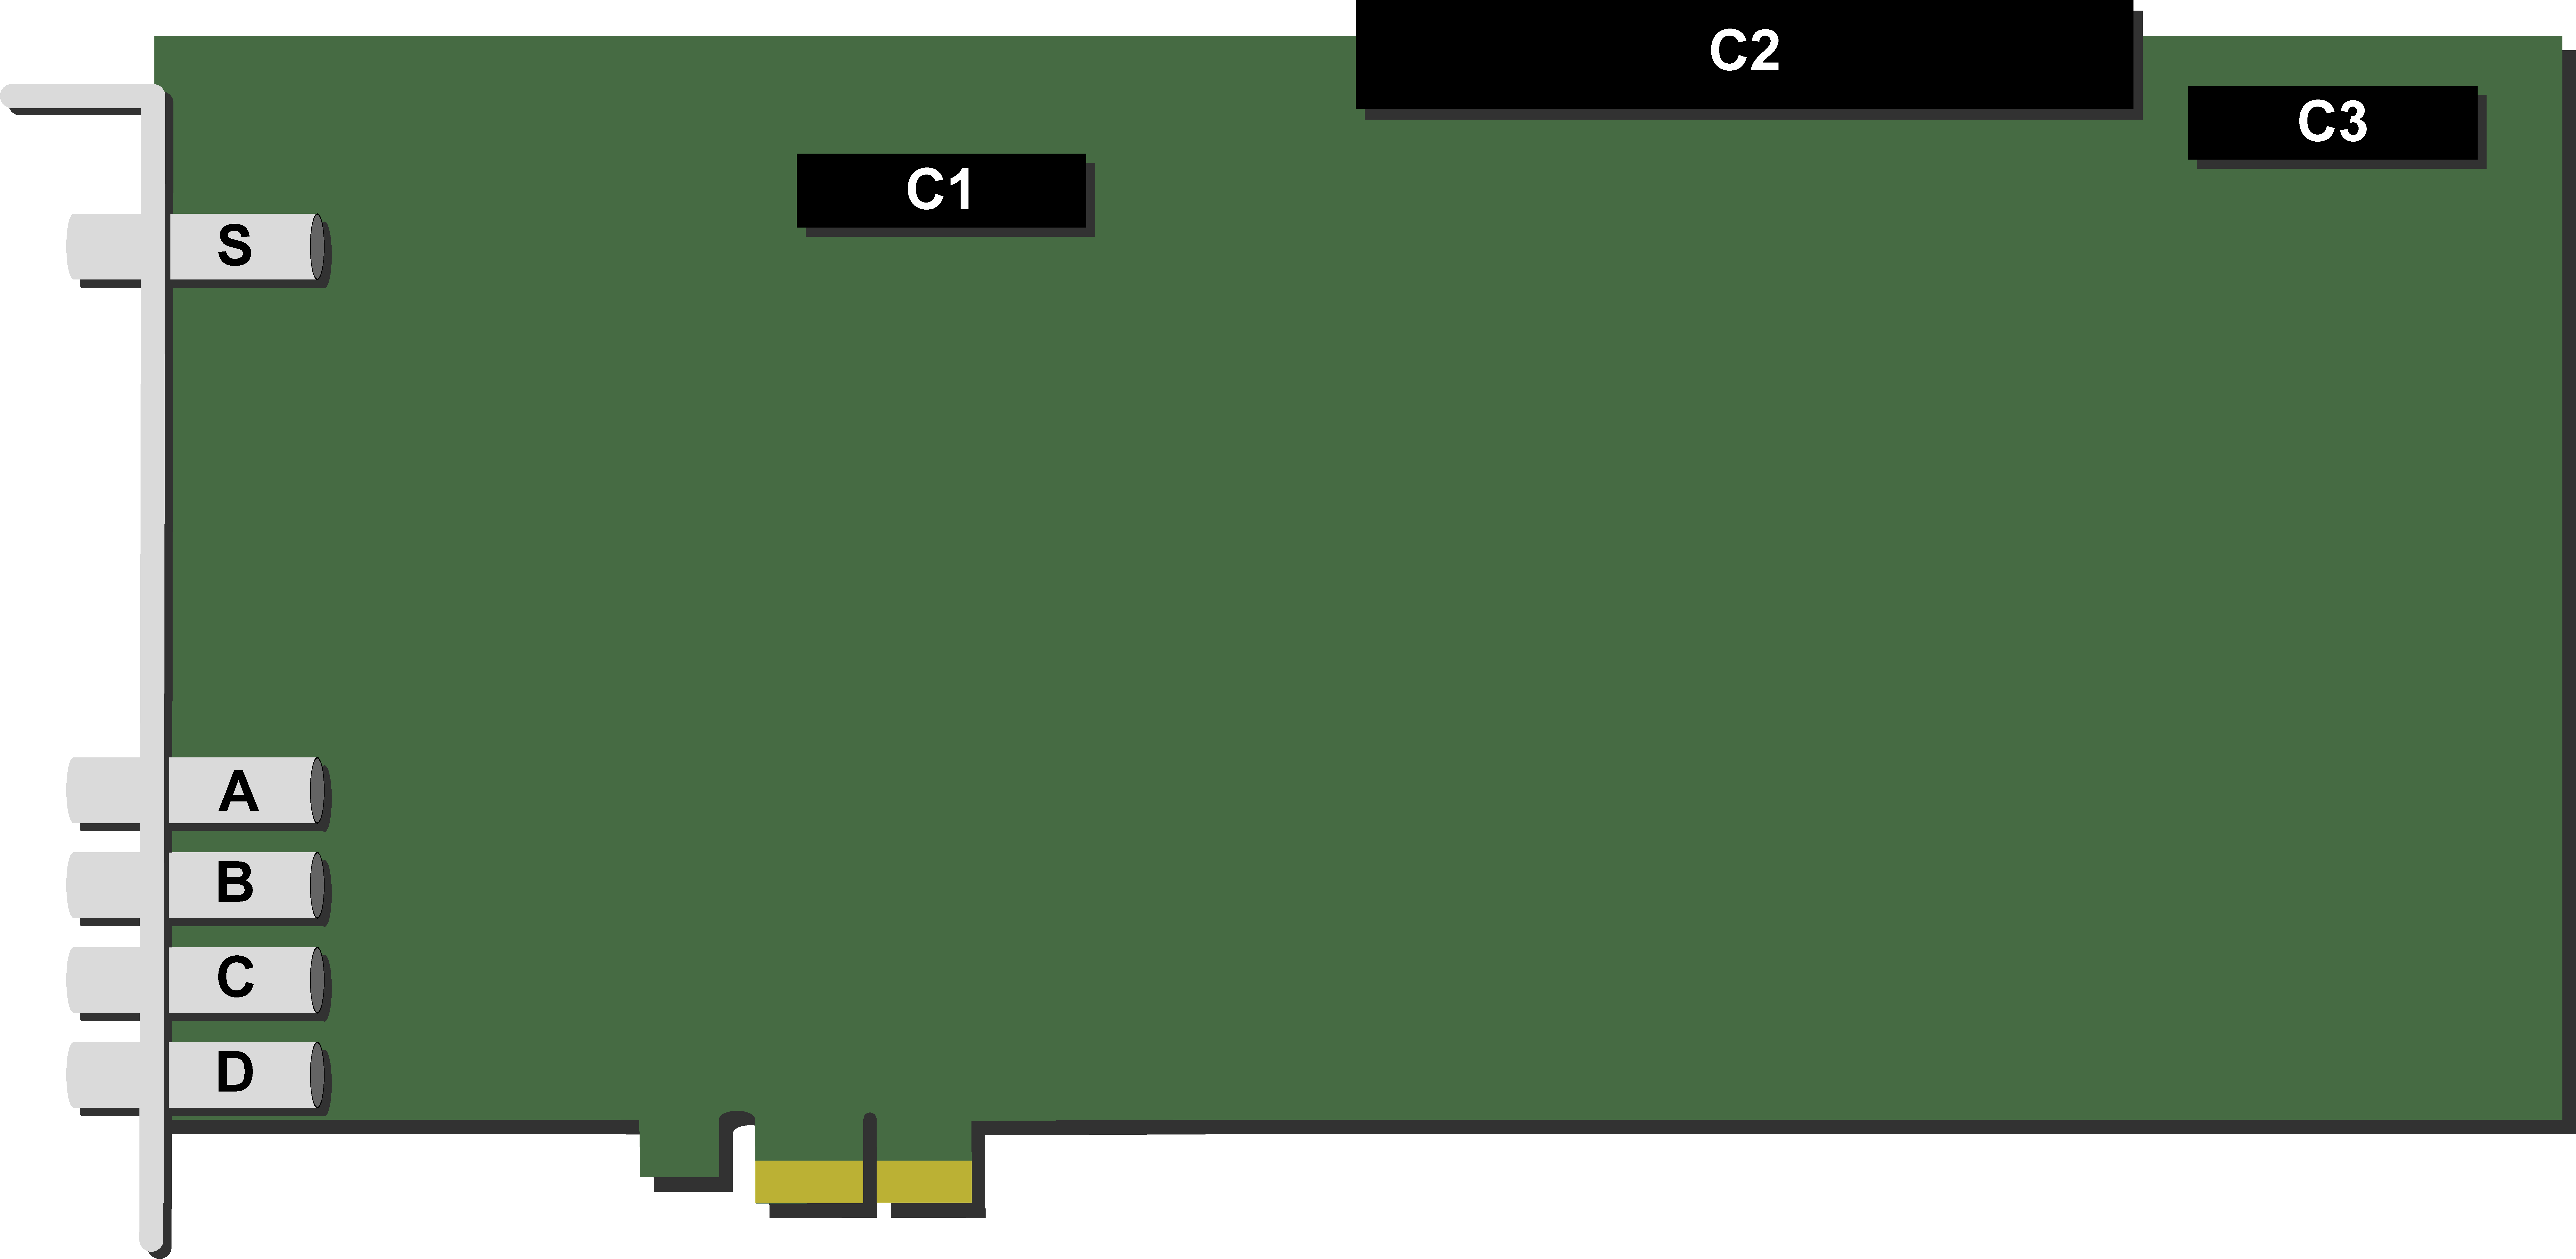
\includegraphics[width=0.7\textwidth]{figures/xTDC4_schematic.pdf}
				\caption{Schematic view of a \deviceName\ board showing inter-board connectors C1, C2 and C3.\label{fig:schematics}}
			\end{center}
		\end{figure*}
	%

	Furthermore, three inter board connectors can be found at the top edge of the \deviceName\ board, as displayed in Figure \ref{fig:schematics} on page \pageref{fig:schematics}. 
	Connector C1 (labelled J25 on the board) is reserved for future use. The pinout of connector C2 (labelled J12 on the board) is shown in Table \ref{con2} and the pinout of connector C3 (labelled as J6 on the board) is depicted in Table \ref{con3}.

	\begin{table}
	\begin{small}
		\begin{center}
			\begin{tabular}{|c|c|}
				\hline
				Pin & Name\\
				\hline\hline
				1, 2 & GND\\
				\hline
				3, 4 & external CLK in N, external CLK in P\\
				\hline
				5, 6 & GND\\
				\hline
				7, 8 & reserved/NC\\
				\hline
				9, 10 & GND\\
				\hline
				11, 12 & reserved/NC\\
				\hline
				13, 14 & GND\\
				\hline
				15, 16 & reserved/NC\\
				\hline
				17, 18 & GND\\
				\hline
				19, 20 & reserved/NC\\
				\hline
				21, 22 & GND\\
				\hline
				23, 24 & reserved/NC\\
				\hline
				25, 26 & GND\\
				\hline
				27, 28 & reserved/NC\\
				\hline
				29, 30 & GND\\
				\hline
				31, 32 & reserved/NC\\
				\hline
				33, 34 & GND\\
				\hline
			\end{tabular}
			\caption{Pinout of connector C2 (J12).}
			\label{con2}
		\end{center}
	\end{small}
	\end{table}

	\begin{table}
	\begin{small}
		\begin{center}
			\begin{tabular}{|c|c|}
				\hline
				Pin & Name\\
				\hline\hline
				1 & +3.3 V\\
				\hline
				2 - 9 & reserved/NC\\
				\hline
				10 & GND\\
				\hline
			\end{tabular}
			\caption{Pinout of connector C3 (J6).}
			\label{con3}
		\end{center}
	\end{small}
	\end{table}

\section{\deviceName\ Functionality}
	The \deviceName\ is a ``classic'' common start time-to-digital converter. 

	\itett{ %TimeTagger Version
		It records the time difference between a leading or trailing edge on the start input to the leading and trailing edges of the stop inputs. 
		Rising and falling edges of the stop channel A-D can be enabled individually. The measurements are quantized to $500$~ps for -2G devices and tp $1000$~ps for -1G devices. 
		The timestamps are recorded in integer multiples of a bin size of $500$~ps for both board types to simplifiy setups where data from differnt board types is combined.
		Transitions of the input signals are called hits. To reliably detect hits the signal has to be stable for more than one quantisation interval before and after the edge.  
		Triggers on the start channel must not occur less than 5ns apart. The \deviceName\ records events without dead time at a readout rate of about 48MHits/s.
	} { %xTDC4 Version
		It records the time difference between leading or trailing edges on the start input and the stop inputs. 
		Each stop channel A-D can be enabled individually. 
		The standard deviation of the timestamps is approx. $8$~ps. 
		The timestamps are recorded in integer multiples of a bin size of $5/(3\cdot 128) = 13.0208\overline{3}$~ps. 
		The data acquisition can be limited to rising or falling signal transitions. 
		
		The maximum trigger rate on the start channel is 4~MHz.
		
		\subsection{Handling of Difficult Hits}
			\label{difficulthits}
			Transitions of the input signals are called hits. To measure all hits with the meximum resolution the hits must fulfill all criteria set forth in this document.
			However, the \deviceName does include mechanisms to provide as much information as possible for hits that fall out of these specs.
		
			To reliably detect hits the signal has to be stable for at least $900$~ps before and after the edge that is to be measured. 
			Pulses as short as $250$~ps are usually detected at full resolution, but have a significant chance to assigned to the wrong group or appeare out of order. 
			For these hits bit 7 in the data word is set. See section \ref{flags} for more information on the data format.

			Between multiple hits on a stop channel a deadtime of approximately $5$~ns is required for full resolution. 
			Hits that are closer together will only be reported with a resolution of $5/6~ns = 833,\overline{3}~ps$. For these hits both bits 6 and 7 are set.

			Data is copied from the 15 entry L0 FIFO to the larger downstream FIFOs at a reate of about 12MHz per channel. 
			If the L0 FIFO overflows the hig resolution measurement of some hits will be discarded. 
			In this case a measurement from an alternative TDC wil be used that has a resolution of about 150ps. 
			For these hits bit 6 in the data word will be set
	}

	\subsection{Grouping and Events}
		In typical applications a start hit is followed by a manifold of hits on e.g. a detector. 
		The hits recorded are managed in groups (which are called ``events'' in some applications). 
		Figure \ref{fig:grouping} shows a corresponding timing diagram. The user can define the range of a group, i.e. the time window within which hits 
		on the stop channels are recorded, in software. Hits occurring outside of that time window are discarded. 
		 Different ranges can be set for each of the 4 stop channels by setting corresponding configuration.channel[n].start and .stop values in the channel configuration. 
		The values need to be set as multiples of the bin size.

	%
		\begin{figure*}[ht]
			\begin{center}
				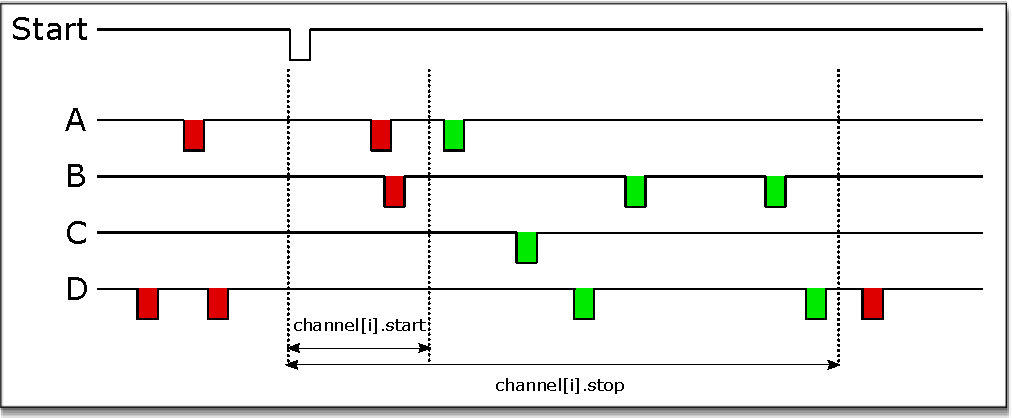
\includegraphics[width=0.7\textwidth]{figures/grouping.pdf}
				\caption{Acquired hits are merged to groups as explained in the text.\label{fig:grouping}}
			\end{center}
		\end{figure*}
	%
	
	\subsection{Auto Triggering Function Generator\label{cp:AutoTriggeringFunctionGenerator}}
		Some applications require internal periodic or random triggering. The \deviceName\ function generator provides this functionality.\par

		The delay between two trigger pulses of this trigger generator is the sum of two components: A fixed value M and a pseudo random value given by the exponent N. \par

		The period is

		\begin{align}
			T = 1 + M + [1...2^N]
		\end{align}

		clock cycles with a duration of $4 ns$ per cycle.\par
		
		The trigger can be used as a source for the TiGer unit (see Section \ref{cp:tiger}).
	
	
	\subsection{Timing Generator (TiGer)\label{cp:tiger}}
		Each LEMO-00 input can be used as a LVCMOS trigger output. The TiGer function can be configured independently for each LEMO-00 connector. 
		Each TiGet block can use an arbitrary combination of inputs to trigger its state machine including the AutoTrigger.
		See Section \ref{cp:tigerblock} for a full description of the configuration options.

		%
		\begin{figure*}[ht]
			\begin{center}
				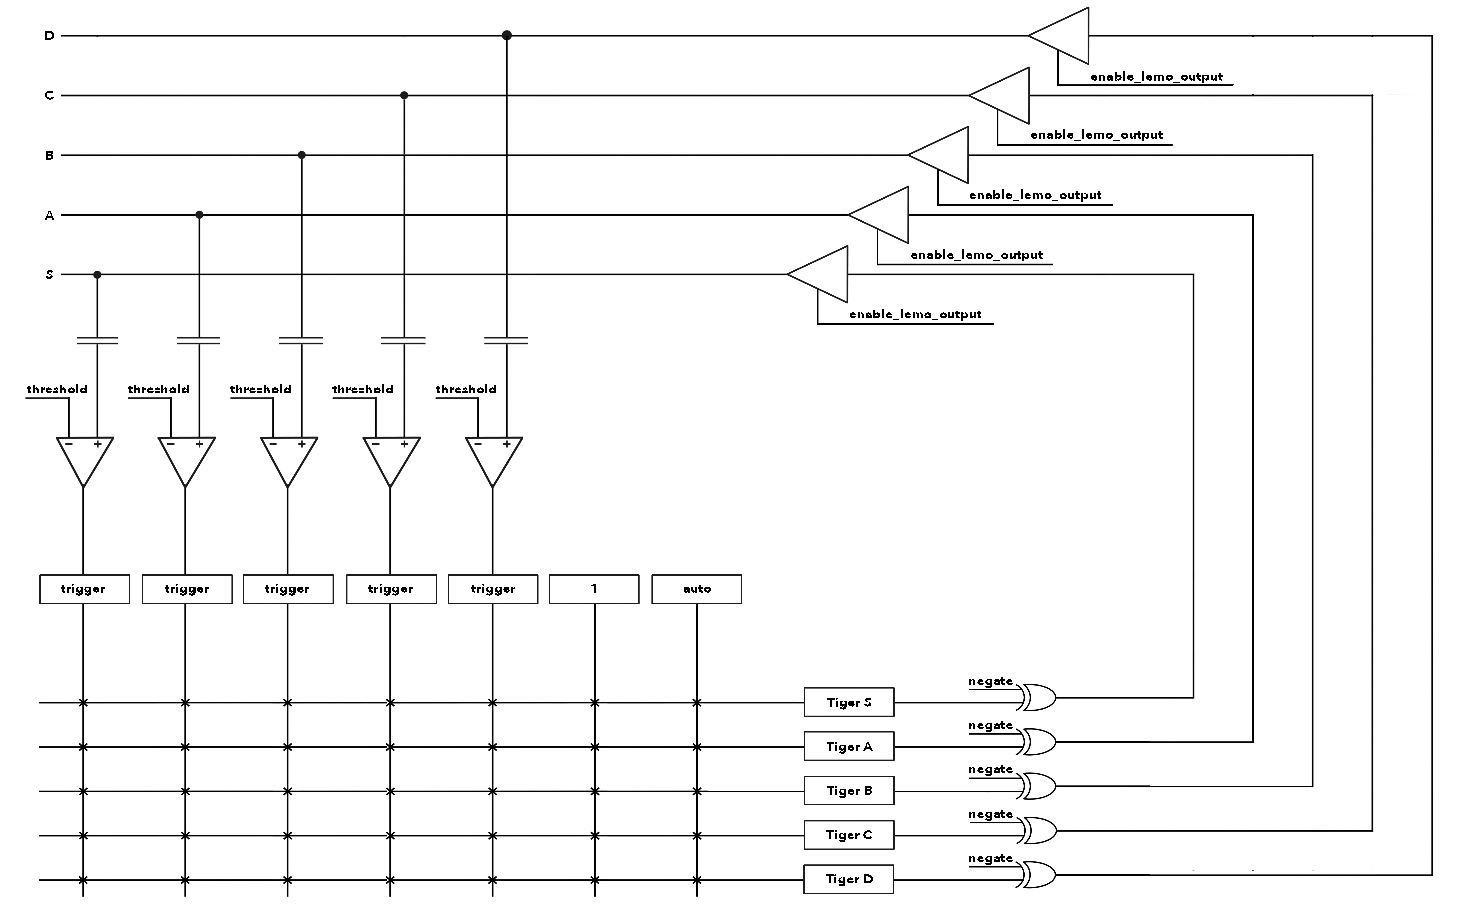
\includegraphics[width=0.7\textwidth]{figures/xTDC4_tiger_matrix.pdf}
				\caption{TiGer blocks can generate outputs that are also available on inputs.\label{fig:matrix}}
			\end{center}
		\end{figure*}
		%

		Figure \ref{fig:matrix} shows how the TiGer blocks are connected. They can be triggered by an OR of an arbitrary combination of inputs, 
		including the auto trigger. Each TiGer can drive its output to its corresponding LEMO connector. This turns the connector into a DC coupled output. 
		Connected hardware must not drive any signals to connectors used as outputs, as doing so could damage both the \deviceName and the external hardware.
		Pulses that are short enough for the input AC coupling are available as input signals to the \deviceName. 
		This can be used to measure exact time differences between the generated output signals and input signals on other channels.

		
		\subsubsection{TiGer Example: Generate 200 kHz Start Pulse}
		The AutoTrigger is used to generate a 200 kHz period. The TiGer generates a 200 kHz signal with $12 ns$ pulse width on LEMO-00 output Start.
\begin{lstlisting}[frame=tlrb]
// generate an internal 200 kHz trigger
config.auto_trigger_period = 1250;
config.auto_trigger_random_exponent = 0;

// setup TiGer
config.tiger_block[0].enable = 1;
config.tiger_block[0].start = 0;
config.tiger_block[0].stop = config.tiger_block[0].start + 2;
config.tiger_block[0].negate = 0;
config.tiger_block[0].enable_lemo_output = 1;
config.tiger_block[0].sources = TIMETAGGER4_TRIGGER_SOURCE_AUTO;

// if TiGer is used for triggering other channels with positive pulses
config.dc_offset[0] = TIMETAGGER4_DC_OFFSET_P_LVCMOS_18; 
\end{lstlisting}

	\subsubsection{TiGer Example: Generate Common-Start from Stops}
	A trigger event on any Stop channel is used to generate the next event on the Start channel. 
	The start value of the TiGer block should be set so that the pulse occurs after the last stop event of the group.
\begin{lstlisting}[frame=tlrb]
config.tiger_block[0].enable = 1;
config.tiger_block[0].start = 32;
config.tiger_block[0].stop = config.tiger_block[0].start + 2;
config.tiger_block[0].negate = 0;
config.tiger_block[0].enable_lemo_output = 1;
// an event on any of the channels A - D starts 
config.tiger_block[0].sources = TIMETAGGER4_TRIGGER_SOURCE_A|TIMETAGGER4_TRIGGER_SOURCE_B|TIMETAGGER4_TRIGGER_SOURCE_C|TIMETAGGER4_TRIGGER_SOURCE_D;

// if TiGer is used for triggering with positive pulses
config.dc_offset[0] = TIMETAGGER4_DC_OFFSET_P_LVCMOS_18; 
\end{lstlisting}
	
